\documentclass[a4paper]{article}
\usepackage[utf8]{inputenc}
\usepackage[spanish, es-tabla, es-noshorthands]{babel}
\usepackage[table,xcdraw]{xcolor}
\usepackage[a4paper, footnotesep = 1cm, width=18cm, left=2cm, top=2.5cm, height=25cm, textwidth=18cm, textheight=25cm]{geometry}
%\geometry{showframe}

\usepackage{tikz}
\usepackage{amsmath}
\usepackage{amsfonts}
\usepackage{amssymb}
\usepackage{float}
\usepackage{graphicx}
\usepackage{caption}
\usepackage{subcaption}
\usepackage{multicol}
\usepackage{multirow}
\setlength{\doublerulesep}{\arrayrulewidth}
\usepackage{booktabs}

\usepackage{hyperref}
\hypersetup{
    colorlinks=true,
    linkcolor=blue,
    filecolor=magenta,      
    urlcolor=blue,
    citecolor=blue,    
}
\newcommand\underrel[2]{\mathrel{\mathop{#2}\limits_{#1}}}
\newcommand{\quotes}[1]{``#1''}
\usepackage{array}
\newcolumntype{C}[1]{>{\centering\let\newline\\\arraybackslash\hspace{0pt}}m{#1}}
\usepackage[american]{circuitikz}
\usetikzlibrary{calc}
\usepackage{fancyhdr}
\usepackage{units} 

\graphicspath{{../Ejercicio-1/}{../Ejercicio-2/}{../Ejercicio-3/}}

\pagestyle{fancy}
\fancyhf{}
\lhead{22.13 Electrónica III}
\rhead{Mechoulam, Lambertucci, Martorell, Londero}
\rfoot{\center \thepage}
\usepackage{tikz}
\usetikzlibrary{matrix,calc}

%isolated term
%#1 - Optional. Space between node and grouping line. Default=0
%#2 - node
%#3 - filling color
\newcommand{\implicantsol}[3][0]{
    \draw[rounded corners=3pt, fill=#3, opacity=0.3] ($(#2.north west)+(135:#1)$) rectangle ($(#2.south east)+(-45:#1)$);
    }


%internal group
%#1 - Optional. Space between node and grouping line. Default=0
%#2 - top left node
%#3 - bottom right node
%#4 - filling color
\newcommand{\implicant}[4][0]{
    \draw[rounded corners=3pt, fill=#4, opacity=0.3] ($(#2.north west)+(135:#1)$) rectangle ($(#3.south east)+(-45:#1)$);
    }

%group lateral borders
%#1 - Optional. Space between node and grouping line. Default=0
%#2 - top left node
%#3 - bottom right node
%#4 - filling color
\newcommand{\implicantcostats}[4][0]{
    \draw[rounded corners=3pt, fill=#4, opacity=0.3] ($(rf.east |- #2.north)+(90:#1)$)-| ($(#2.east)+(0:#1)$) |- ($(rf.east |- #3.south)+(-90:#1)$);
    \draw[rounded corners=3pt, fill=#4, opacity=0.3] ($(cf.west |- #2.north)+(90:#1)$) -| ($(#3.west)+(180:#1)$) |- ($(cf.west |- #3.south)+(-90:#1)$);
}

%group top-bottom borders
%#1 - Optional. Space between node and grouping line. Default=0
%#2 - top left node
%#3 - bottom right node
%#4 - filling color
\newcommand{\implicantdaltbaix}[4][0]{
    \draw[rounded corners=3pt, fill=#4, opacity=0.3] ($(cf.south -| #2.west)+(180:#1)$) |- ($(#2.south)+(-90:#1)$) -| ($(cf.south -| #3.east)+(0:#1)$);
    \draw[rounded corners=3pt, fill=#4, opacity=0.3] ($(rf.north -| #2.west)+(180:#1)$) |- ($(#3.north)+(90:#1)$) -| ($(rf.north -| #3.east)+(0:#1)$);
}

%group corners
%#1 - Optional. Space between node and grouping line. Default=0
%#2 - filling color
\newcommand{\implicantcantons}[2][0]{
    \draw[rounded corners=3pt, opacity=.3] ($(rf.east |- 0.south)+(-90:#1)$) -| ($(0.east |- cf.south)+(0:#1)$);
    \draw[rounded corners=3pt, opacity=.3] ($(rf.east |- 8.north)+(90:#1)$) -| ($(8.east |- rf.north)+(0:#1)$);
    \draw[rounded corners=3pt, opacity=.3] ($(cf.west |- 2.south)+(-90:#1)$) -| ($(2.west |- cf.south)+(180:#1)$);
    \draw[rounded corners=3pt, opacity=.3] ($(cf.west |- 10.north)+(90:#1)$) -| ($(10.west |- rf.north)+(180:#1)$);
    \fill[rounded corners=3pt, fill=#2, opacity=.3] ($(rf.east |- 0.south)+(-90:#1)$) -|  ($(0.east |- cf.south)+(0:#1)$) [sharp corners] ($(rf.east |- 0.south)+(-90:#1)$) |-  ($(0.east |- cf.south)+(0:#1)$) ;
    \fill[rounded corners=3pt, fill=#2, opacity=.3] ($(rf.east |- 8.north)+(90:#1)$) -| ($(8.east |- rf.north)+(0:#1)$) [sharp corners] ($(rf.east |- 8.north)+(90:#1)$) |- ($(8.east |- rf.north)+(0:#1)$) ;
    \fill[rounded corners=3pt, fill=#2, opacity=.3] ($(cf.west |- 2.south)+(-90:#1)$) -| ($(2.west |- cf.south)+(180:#1)$) [sharp corners]($(cf.west |- 2.south)+(-90:#1)$) |- ($(2.west |- cf.south)+(180:#1)$) ;
    \fill[rounded corners=3pt, fill=#2, opacity=.3] ($(cf.west |- 10.north)+(90:#1)$) -| ($(10.west |- rf.north)+(180:#1)$) [sharp corners] ($(cf.west |- 10.north)+(90:#1)$) |- ($(10.west |- rf.north)+(180:#1)$) ;
}

%Empty Karnaugh map 4x4
\newenvironment{Karnaugh}%
{
\begin{tikzpicture}[baseline=(current bounding box.north),scale=0.8]
\draw (0,0) grid (4,4);
\draw (0,4) -- node [pos=0.7,above right,anchor=south west] {ba} node [pos=0.7,below left,anchor=north east] {dc} ++(135:1);
%
\matrix (mapa) [matrix of nodes,
        column sep={0.8cm,between origins},
        row sep={0.8cm,between origins},
        every node/.style={minimum size=0.3mm},
        anchor=8.center,
        ampersand replacement=\&] at (0.5,0.5)
{
                       \& |(c00)| 00         \& |(c01)| 01         \& |(c11)| 11         \& |(c10)| 10         \& |(cf)| \phantom{00} \\
|(r00)| 00             \& |(0)|  \phantom{0} \& |(1)|  \phantom{0} \& |(3)|  \phantom{0} \& |(2)|  \phantom{0} \&                     \\
|(r01)| 01             \& |(4)|  \phantom{0} \& |(5)|  \phantom{0} \& |(7)|  \phantom{0} \& |(6)|  \phantom{0} \&                     \\
|(r11)| 11             \& |(12)| \phantom{0} \& |(13)| \phantom{0} \& |(15)| \phantom{0} \& |(14)| \phantom{0} \&                     \\
|(r10)| 10             \& |(8)|  \phantom{0} \& |(9)|  \phantom{0} \& |(11)| \phantom{0} \& |(10)| \phantom{0} \&                     \\
|(rf) | \phantom{00}   \&                    \&                    \&                    \&                    \&                     \\
};
}%
{
\end{tikzpicture}
}

%Empty Karnaugh map 2x4
\newenvironment{Karnaughvuit}%
{
\begin{tikzpicture}[baseline=(current bounding box.north),scale=0.8]
\draw (0,0) grid (4,2);
\draw (0,2) -- node [pos=0.7,above right,anchor=south west] {bc} node [pos=0.7,below left,anchor=north east] {a} ++(135:1);
%
\matrix (mapa) [matrix of nodes,
        column sep={0.8cm,between origins},
        row sep={0.8cm,between origins},
        every node/.style={minimum size=0.3mm},
        anchor=4.center,
        ampersand replacement=\&] at (0.5,0.5)
{
                      \& |(c00)| 00         \& |(c01)| 01         \& |(c11)| 11         \& |(c10)| 10         \& |(cf)| \phantom{00} \\
|(r00)| 0             \& |(0)|  \phantom{0} \& |(1)|  \phantom{0} \& |(3)|  \phantom{0} \& |(2)|  \phantom{0} \&                     \\
|(r01)| 1             \& |(4)|  \phantom{0} \& |(5)|  \phantom{0} \& |(7)|  \phantom{0} \& |(6)|  \phantom{0} \&                     \\
|(rf) | \phantom{00}  \&                    \&                    \&                    \&                    \&                     \\
};
}%
{
\end{tikzpicture}
}

%Empty Karnaugh map 2x2
\newenvironment{Karnaughquatre}%
{
\begin{tikzpicture}[baseline=(current bounding box.north),scale=0.8]
\draw (0,0) grid (2,2);
\draw (0,2) -- node [pos=0.7,above right,anchor=south west] {b} node [pos=0.7,below left,anchor=north east] {a} ++(135:1);
%
\matrix (mapa) [matrix of nodes,
        column sep={0.8cm,between origins},
        row sep={0.8cm,between origins},
        every node/.style={minimum size=0.3mm},
        anchor=2.center,
        ampersand replacement=\&] at (0.5,0.5)
{
          \& |(c00)| 0          \& |(c01)| 1  \\
|(r00)| 0 \& |(0)|  \phantom{0} \& |(1)|  \phantom{0} \\
|(r01)| 1 \& |(2)|  \phantom{0} \& |(3)|  \phantom{0} \\
};
}%
{
\end{tikzpicture}
}

%Defines 8 or 16 values (0,1,X)
\newcommand{\contingut}[1]{%
\foreach \x [count=\xi from 0]  in {#1}
     \path (\xi) node {\x};
}

%Places 1 in listed positions
\newcommand{\minterms}[1]{%
    \foreach \x in {#1}
        \path (\x) node {1};
}

%Places 0 in listed positions
\newcommand{\maxterms}[1]{%
    \foreach \x in {#1}
        \path (\x) node {0};
}

%Places X in listed positions
\newcommand{\indeterminats}[1]{%
    \foreach \x in {#1}
        \path (\x) node {X};
}

% \begin{document}
%     \begin{Karnaugh}
%         \contingut{0,0,0,0,0,0,0,0,0,0,0,0,0,0,0,0}
%        \implicant{0}{2}{red}
%        \implicant{5}{15}{purple}
%        \implicantdaltbaix[3pt]{3}{10}{blue}
%     \implicantcantons[2pt]{orange}
%        \implicantcostats{4}{14}{green}
%     \end{Karnaugh}
%     %
%     \begin{Karnaughvuit}
%        \minterms{3,4}
%         \maxterms{0,1,6,7}
%        \indeterminats{2,5}
%        \implicant{3}{2}{green}
%        \implicant{4}{5}{}
%     \end{Karnaughvuit}
%     %
%     \begin{Karnaughquatre}
%         \minterms{1,2}
%        \maxterms{0,3}
%        \implicantsol{1}{green}
%        \implicantsol{2}{red}
%     \end{Karnaughquatre}

% \end{document}
\begin{document}

\subsection{Introducción}

Se quiso implementar la siguiente máquina de estados finitos:

\begin{figure}[H]
\centering
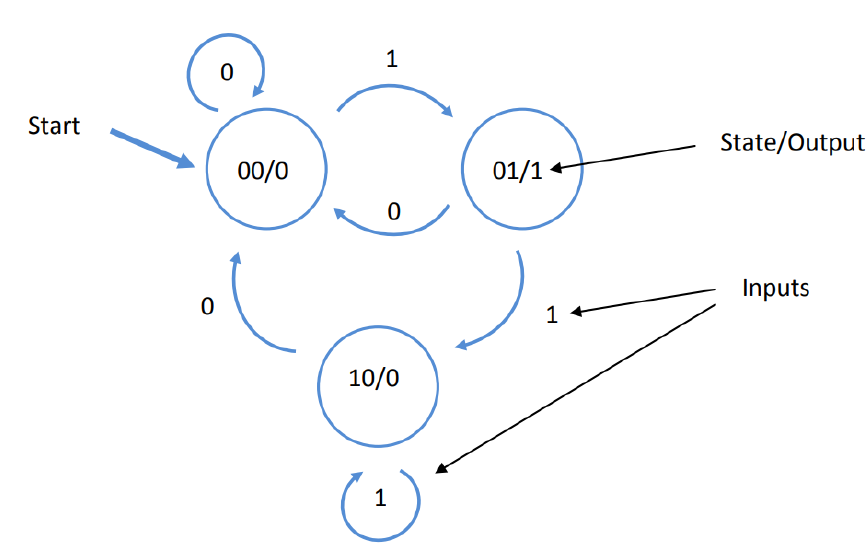
\includegraphics[width=0.6\textwidth]{ImagenesEjercicio3/fsm.png}
\caption{Máquina de estados finitos a implementar.}
\label{fig:fsm}
\end{figure} 

Para esto, se conformó la tabla de estados considerando al estado $00$ como el inicial, resultando:

\begin{table}[H]
\centering
\begin{tabular}{|c|l|c|l|c|l|c|}
\hline
\multicolumn{2}{|c|}{\multirow{2}{*}{$Present State$}} & \multicolumn{4}{c|}{$Next State$} & \multirow{3}{*}{$Output (z)$} \\ \cline{3-6}
\multicolumn{2}{|c|}{} & \multicolumn{2}{c|}{$w=0$} & \multicolumn{2}{c|}{$w=1$} &  \\
\multicolumn{2}{|c|}{$y_2 y_1$} & \multicolumn{2}{c|}{$Y_2Y_1$} & \multicolumn{2}{c|}{$Y_2Y_1$} &  \\ \hline
\multicolumn{2}{|c|}{00} & \multicolumn{2}{c|}{00} & \multicolumn{2}{c|}{01} & 0 \\ \hline
\multicolumn{2}{|c|}{01} & \multicolumn{2}{c|}{00} & \multicolumn{2}{c|}{10} & 1 \\ \hline
\multicolumn{2}{|c|}{10} & \multicolumn{2}{c|}{00} & \multicolumn{2}{c|}{10} & 0 \\ \hline
\multicolumn{2}{|c|}{11} & \multicolumn{2}{c|}{xx} & \multicolumn{2}{c|}{xx} & x \\ \hline
\end{tabular}
\caption{Tabla de estados para la máquina de estados finita a implementar.}
\label{fig:tablaestados}
\end{table}

Como fue necesario implementar tres estados se requirió utilizar dos flip-flops. Luego, se hallaron las fórmulas lógicas para los estados siguientes utilizando mapas de karnaugh.

\begin{figure}[H]
\begin{subfigure}{0.49\textwidth}
\begin{centering}
    \begin{Karnaughvuit}
        \minterms{5, 6}
        \maxterms{0,1,2,4}
        \indeterminats{7, 3}
        
        \implicant{5}{7}{orange}
        \implicant{7}{6}{blue}
        
    \end{Karnaughvuit}
\par\end{centering}
\begin{equation*}
Y_2 = wy_1+wy_2
\end{equation*}
\begin{table}[H]
\caption{Solución para $Y_2.$}
\label{mapa:Y2}
\end{table}
\end{subfigure}
\begin{subfigure}{0.49\textwidth}
\begin{centering}
    \begin{Karnaughvuit}
        \minterms{4}
        \maxterms{0,1,2,5,6}
        \indeterminats{7,3}
        
        \implicantsol{4}{green}
        
    \end{Karnaughvuit}
\par\end{centering}
\begin{equation*}
Y_1 = w(\overline{y_2}\cdot \overline{y_1})
\end{equation*}
\begin{table}[H]
\caption{Solución para $Y_1.$}
\label{mapa:Y1}
\end{table}
\end{subfigure}
\caption{Mapas de Karnaugh para los próximos estados de la maquina de estados finitos.}
\end{figure}

Utilizando el teorema de DeMorgan y simplificando se obtienen dos posibles implementaciones análogas:
\begin{figure}[H]
\begin{subfigure}{0.49\textwidth}
\vspace*{-0.17cm}
\begin{equation*}
\left.\left\{
\begin{aligned}
		& Y_1 = w(\overline{y_2}\cdot \overline{y_1})	 \\		
		& Y_2 = w\overline{(\overline{y_2}\cdot \overline{y_1})}\\		
\end{aligned}
\right.\right\}
\end{equation*}
\caption{Implementación con NAND.}
\end{subfigure}
\begin{subfigure}{0.49\textwidth}
\begin{equation*}
\left.\left\{
\begin{aligned}
		& Y_1 = w(\overline{y_2+y_1}) \\		
		& Y_2 = w(y_2+y_1)\\		
\end{aligned}
\right.\right\}
\end{equation*}
\caption{Implementación con AND y NOR.}
\end{subfigure}
\end{figure}

Si este circuito fuese trabajado directamente sobre el silicio, se elegiría la implementación con NAND ya que sería la más simple de realizar. Sin embargo, como se contruirá un PCB, se decidió utilizar la implementación con AND y NOR ya que se deberían de utilizar solamente dos integrados para el circuito lógico de entrada y salida, a diferencia de la implementación con NAND, que requeriría de tres integrados (utilizando un total de nueve NAND's). Finalmente, a partir de las ecuaciones obtenidas se esquematizó la implementación teórica.

\begin{figure}[H]
	\hspace*{1cm}
	\centering
	\begin{circuitikz}
		\draw
			
			(0,0)
			node[fourport](FF1){}
				(FF1.1) ++ (0.12,0) node[]{\scalebox{1.2}{\rotatebox{-90}{$\triangle$}}}
				 ++ (-0.12,0) node[](FF1_CLK){}
				(FF1.2) ++ (-0.25, 0) node[](){$\overline{y_1}$}
				node[](FF1_2){}
				(FF1.3) ++ (-0.25, 0) node[](){$y_1$}
				node[](FF1_3){}
				(FF1.4) ++ (0.25, 0) node[](){$Y_1$}
				node[](FF1_4){}
				(FF1_CLK) to[short] ++ (-0.5, 0)
					node[](FF1_CLK){}
				(FF1.3) to[short] ++ (0.5, 0)
					node[](FF1_y){}
				(FF1.4) to[short] ++ (-0.5, 0)
					node[](FF1_Y){}
					
				
			(0,-3)
			node[fourport](FF2){}
				(FF2.1) ++ (0.12,0) node[]{\scalebox{1.2}{\rotatebox{-90}{$\triangle$}}}
				 ++ (-0.12,0) node[](FF2_CLK){}
				(FF2.2) ++ (-0.25, 0) node[](){$\overline{y_2}$}
				node[](FF2_-y){}
				(FF2.3) ++ (-0.25, 0) node[](){$y_2$}
				node[](FF2_y){}
				(FF2.4) ++ (0.25, 0) node[](){$Y_2$}
				node[](FF2_Y){}
				(FF2_CLK) to[short] ++ (-0.5, 0)
					node[](FF2_CLK){}
				(FF2.2) to[short] ++ (0.5, 0)
					node[](FF2_-y){}
				(FF2.3) to[short] ++ (1, 0)
					node[](FF2_y){}
				(FF2.4) to[short] ++ (-0.5, 0)
					node[](FF2_Y){}		
					
					
			(-4, -4)node[ocirc, label=west:$CLK$](CLK){}
				(CLK) to[short] ++ (2.5,0) |-(FF2_CLK.center)
				(CLK) to[open, -*]++(2.5, 0.55) |-(FF1_CLK.center)
				
			(FF1_Y) ++ (-0.5, 0) node[and port, xscale=0.7, yscale=0.7](and1){}
			(and1.in 1) ++ (-0.5, 0) node[nor port, xscale=0.7, yscale=0.7](nor1){}
			
			(FF2_Y) ++ (-0.5, 0) node[and port, xscale=0.7, yscale=0.7](and2){}
			(and2.in 2) ++ (-0.5, 0) node[nor port, xscale=0.7, yscale=0.7](nor2){}
			(and2.in 2) ++ (-2, 0) node[nor port, xscale=0.7, yscale=0.7](nor3){}
		
			(-4, -1)node[ocirc, label=west:$w$](w){}
			(w)-|(and1.in 2)
			(w)-|(and2.in 1)
			
			(nor2.in 1) -- (nor2.in 2)
			(nor2.in 1) to[open, -*] ++ (0, -0.2) -- (nor3.out)
			(and2.in 2) -- (nor2.out)
			(and1.in 1) -- (nor1.out)
			(and1.out) -- (FF1_Y.center)
			(and2.out) -- (FF2_Y.center)
			
			(4, -1.5) node[and port, xscale=0.7, yscale=0.7](andout){}
			(FF2_-y) to[short]++(1, 0) |- (andout.in 2)

			(FF1_y)to[short]++(0, 1)to[short]++(-8,0)
				to[short, -*]++(0, -0.6)node[](aux){}
				(aux.center)--(nor1.in 1)
				(aux.center)|-(nor3.in 1)
				
			(FF2_y)to[short]++(0, -2)to[short]++(-8,0)|-(nor3.in 2)
			++(-0.25, 0) node[circ]{} |- (nor1.in 2)
			
			(FF1_y.center)node[circ]{}to[short]++(1, 0)|-(andout.in 1)
			(andout.out)to[short, -o] ++ (0.5, 0) node[label=east:$z$]{}
		;
	\end{circuitikz}
	\caption{Implementación teórica de la lógica de entrada, estados y lógica de salida de la máquina de estados finitos a implementar.}
\end{figure}

\subsection{Simulación}

Se simuló la implementación obtenida en la sección anterior utilizando $Verilog$, un lenguaje descriptivo de hardware y $GTKWave$, un visualizador de señales.

\subsection{Implementación}
Para esta etapa se debió tener un cuidado especial dado que era un requisito en la implementación que la lógica interna del circuito funcione con $3.3V$ mientras que las entradas y salidas debían operar con $5V$.
\subsubsection{Level Shifting}
Para la conversión de $3V3$ a $5V$ de la salida se decidió utilizar un trasistor bipolar NPN como indica la Figura (\ref{circ:stepup}). Luego, para la entradas, las cuales debían pasar de $5V$ a $3V3$ se utilizó un diodo zener de $3V3$ con una resistencia limitadora de corriente calculada conociendo la corriente de codo del diodo y la corriente de entrada de las compuertas de tecnología CMOS utilizadas. Esta implementación se puede observar en la Figura(\ref{circ:stepdown}). 

\begin{figure}[H]

	\centering
	\begin{subfigure}{0.49\textwidth}
		\centering
		\begin{circuitikz}
			\draw
			(0,0)
			node[ocirc, label=west:$In$](in){}
			++(2, 0) node[npn, rotate=-90](npn){}
			(npn.B) ++ (0, 2)node[ocirc, label=north:$3V3$](3v3){}
			(3v3)to[R=$2k2$]++(0, -2)
			(3v3)++(2, 0)node[ocirc, label=north:$5V$](5v){}
			(5v)to[R=$6k8$]++(0, -2)to[short, -*]++(0, -0.83)
			(npn.C) to[short]++(2.5, 0)node[ocirc, label=east:$Out$]{}
			(npn.E)--(in.center)			
			;
		\end{circuitikz}
		\caption{\centering Transistor BJT NPN en configuración base común utilizado como step-up level-shifter.}
		\label{circ:stepup}
	\end{subfigure}
	\begin{subfigure}{0.49\textwidth}
	\centering
	\begin{circuitikz}
			\draw
				(0,0)
				node[ocirc, label=west:$In$]{}
				to[R, l^=$100\Omega$]++(2.5,0)
				to[open]++(0, -2)
				node[tlground]{}
				to[full ZZener diode, l_=$3V3$, -*] ++ (0, 2)
				
				to[short] ++ (1, 0)
				node[ocirc, label=east:$Out$]{}
				%%%%%%%%%%%%%%%%%%%%%%%%%%
				to[open]++(0, 1.45)
			;
		\end{circuitikz}
		\caption{\centering Regulador de tensión de $3V3$ con diodo zener y resistencia utilizado como step-down level-shifter.}
		\label{circ:stepdown}
	\end{subfigure}

\end{figure}

\subsubsection{Diseño Final}

Finalmente se presenta a continuación el diseño final de la máquina de estados finitos implementada.

\begin{figure}[H]
	\hspace*{-0.6cm}
	\centering
	\scalebox{0.85}{
	\begin{circuitikz}
		\draw
			
			(0,0)
			node[fourport](FF1){}
				(FF1.1) ++ (0.12,0) node[]{\scalebox{1.2}{\rotatebox{-90}{$\triangle$}}}
				 ++ (-0.12,0) node[](FF1_CLK){}
				(FF1.2) ++ (-0.25, 0) node[](){$\overline{y_1}$}
				node[](FF1_2){}
				(FF1.3) ++ (-0.25, 0) node[](){$y_1$}
				node[](FF1_3){}
				(FF1.4) ++ (0.25, 0) node[](){$Y_1$}
				node[](FF1_4){}
				(FF1_CLK) to[short] ++ (-0.5, 0)
					node[](FF1_CLK){}
				(FF1.3) to[short] ++ (0.5, 0)
					node[](FF1_y){}
				(FF1.4) to[short] ++ (-0.5, 0)
					node[](FF1_Y){}
					
				
			(0,-3)
			node[fourport](FF2){}
				(FF2.1) ++ (0.12,0) node[]{\scalebox{1.2}{\rotatebox{-90}{$\triangle$}}}
				 ++ (-0.12,0) node[](FF2_CLK){}
				(FF2.2) ++ (-0.25, 0) node[](){$\overline{y_2}$}
				node[](FF2_-y){}
				(FF2.3) ++ (-0.25, 0) node[](){$y_2$}
				node[](FF2_y){}
				(FF2.4) ++ (0.25, 0) node[](){$Y_2$}
				node[](FF2_Y){}
				(FF2_CLK) to[short] ++ (-0.5, 0)
					node[](FF2_CLK){}
				(FF2.2) to[short] ++ (0.5, 0)
					node[](FF2_-y){}
				(FF2.3) to[short] ++ (1, 0)
					node[](FF2_y){}
				(FF2.4) to[short] ++ (-0.5, 0)
					node[](FF2_Y){}		
					
					
			(-4, -4)node[label=north:$CLK'$](CLK){}
				(CLK) to[short] ++ (2.5,0) |-(FF2_CLK.center)
				(CLK) to[open, -*]++(2.5, 0.55) |-(FF1_CLK.center)
				
			(FF1_Y) ++ (-0.5, 0) node[and port, xscale=0.7, yscale=0.7](and1){}
			(and1.in 1) ++ (-0.5, 0) node[nor port, xscale=0.7, yscale=0.7](nor1){}
			
			(FF2_Y) ++ (-0.5, 0) node[and port, xscale=0.7, yscale=0.7](and2){}
			(and2.in 2) ++ (-0.5, 0) node[nor port, xscale=0.7, yscale=0.7](nor2){}
			(and2.in 2) ++ (-2, 0) node[nor port, xscale=0.7, yscale=0.7](nor3){}
		
			(-4, -1)node[label=north:$w'$](w){}
			(w)-|(and1.in 2)
			(w)-|(and2.in 1)
			
			(nor2.in 1) -- (nor2.in 2)
			(nor2.in 1) to[open, -*] ++ (0, -0.2) -- (nor3.out)
			(and2.in 2) -- (nor2.out)
			(and1.in 1) -- (nor1.out)
			(and1.out) -- (FF1_Y.center)
			(and2.out) -- (FF2_Y.center)
			
			(4, -1.5) node[and port, xscale=0.7, yscale=0.7](andout){}
			(FF2_-y) to[short]++(1, 0) |- (andout.in 2)

			(FF1_y)to[short]++(0, 1)to[short]++(-8,0)
				to[short, -*]++(0, -0.6)node[](aux){}
				(aux.center)--(nor1.in 1)
				(aux.center)|-(nor3.in 1)
				
			(FF2_y)to[short]++(0, -2)to[short]++(-8,0)|-(nor3.in 2)
			++(-0.25, 0) node[circ]{} |- (nor1.in 2)
			
			(FF1_y.center)node[circ]{}to[short]++(1, 0)|-(andout.in 1)
			(andout.out)to[short] ++ (0.5, 0) node[label=north:$z'$]{}

			
			(andout.out)
			node[](in){}
			++(1.5, 0) node[npn, rotate=-90](npn){}
			(npn.B) ++ (0, 2)node[](3v3){}
			(3v3)to[R=$2k2$]++(0, -2)
			(3v3)++(2, 0)node[](5v){}
			(5v)to[R=$6k8$]++(0, -2)to[short, -*]++(0, -0.83)
			(npn.C) to[short]++(2.5, 0)node[ocirc, label=east:$z$]{}
			(npn.E)--(in.center)
						
			(w)++(-7, 0)			
				node[label=west:$w$]{}
				to[R, l^=$100\Omega$]++(3,0)
				to[open]++(0, -2)
				node[tlground]{}
				to[full ZZener diode, l_=$3V3$, -*] ++ (0, 2)
				to[short]++(4.12,0)
				
			(CLK)++(-7, 0)			
				node[label=west:$CLK$]{}
				to[R, l^=$100\Omega$]++(3,0)
				to[open]++(0, -2)
				node[tlground]{}
				to[full ZZener diode, l_=$3V3$, -*] ++ (0, 2)
				to[short]++(4.12,0)
				
			(w) ++ (0, 3) ++(-7, 0)			
				node[label=west:$5V$]{}
				to[R, l^=$100\Omega$]++(3,0)
				to[open]++(0, -2)
				node[tlground]{}
				to[full ZZener diode, l_=$3V3$, -*] ++ (0, 2)
				node[](aux2){}
				to[short]++(0, 0.5)
				to[open]++(0, -0.5)
				to[short]++(13.62,0)
				to[short]++(0, -0.65)
				(aux2)to[short]++(0, 0.75)to[short]++(1, 0)node[ocirc, label=east:$3V3$]{}
			(w) ++ (0, 3) ++(-6.5, 0) to[short]++(0, 1.5)to[short]++(18.12, 0)to[short]++(0, -2.15)
		;
	\end{circuitikz}
	}
	\caption{Implementación de la máquina de estados finitos junto a la conversión de niveles de tensión.}
\end{figure}

\subsubsection{Componentes}
A continuación se detallan los componentes utilizados en la implementación:
\begin{itemize}
\item Dual Flip-flop D: \href{http://www.ti.com/lit/ds/symlink/cd4013b.pdf}{CD4013}
\item Quad 2-input AND: \href{https://www.mouser.com/datasheet/2/308/74HC08.REV1-102589.pdf}{74HC02}
\item Quad 2-input NOR: \href{https://assets.nexperia.com/documents/data-sheet/74HC_HCT02.pdf}{74HC02}
\item BJT NPN: \LARGE{FALTA}
\item Diodo Zener 3V3: \LARGE{FALTA}
\end{itemize}

\subsection{Mediciones}

\subsection{Conclusiones}


\end{document}